\documentclass[12pt,fleqn]{article}\usepackage{../common}
\begin{document}
Yaklasiksal SVD ile Tavsiye Sistemleri

{\em SVD, Toplu Tavsiye} yazisinda Movielens verisine SVD uygulayarak once
boyut azaltmistik. Azaltilmis boyut uzerinden, yeni bir kullanicinin diger
mevcut kullanicilara mesafesini hesaplamis, ve boylece en cok benzedigi
diger kullaniciyi bulmustuk. Bu kullanicinin bir film icin verdigi notu yeni
kullanici icin tahmin olarak baz aldik. 

SVD uygulamanin degisik bir yolu daha var. Netflix yarismasinda kullanilan
[1] bir yaklasim soyle. Alttaki SVD ayristirmasina bakalim, 

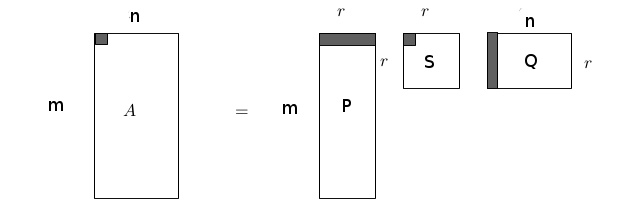
\includegraphics[height=4cm]{svdapprox_1.png}

1. kullanicini 1. filme verdigi not ustte gosterilen satirlarin carpimi
ile, eger ufak harfler ve kullanici (user) icin $u$, film icin $i$ indisini
kullanirsak, ve $q,p$ vektorlerini $Q,P$ matrislerinin sirasiyla kolon ve
satirlarini gostermek icin kullanirsak, ayristirma sonrasi begeni degerinin
onemli bir kismi $q_i^Tp_u$ carpimindadir.



$$
\min_{b*,q*,p*} \sum_{u,i} (r_{ui} - \mu + b_i + b_u + q_i^Tp_u)^2 + 
\lambda_4 (b_i^2 + b_u^2 + ||q_i||^2 + ||p_u||^2)
$$
$$
\hat{r}_{ui} = \mu + b_i + b_u + q_i^Tp_u
$$

$$
\min_{b*,q*,p*} \sum_{u,i} (r_{ui} - \hat{r}_{ui})^2 + 
\lambda_4 (b_i^2 + b_u^2 + ||q_i||^2 + ||p_u||^2)
$$

$$ e_{ui} := r_{ui} - \hat{r}_{ui} $$

$$
b_u \leftarrow b_u + \gamma (e_{ui} - \lambda \cdot b_u)
$$

$$
b_i \leftarrow b_i + \gamma (e_{ui} - \lambda \cdot b_i)
$$

$$
q_i \leftarrow q_i + \gamma (e_{ui}\cdot p_u - \lambda \cdot q_i)
$$

$$
p_u \leftarrow p_u + \gamma (e_{ui}\cdot q_i - \lambda \cdot p_u)
$$




\begin{minted}[fontsize=\footnotesize]{python}
import pandas as pd
import ssvd; reload(ssvd)
d =  np.array(
[[  5.,   5.,   3.,  nan,   5.,   5.],
 [  5.,  nan,   4.,  nan,   4.,   4.],
 [ nan,   3.,  nan,   5.,   4.,   5.],
 [  5.,   4.,   3.,   3.,   5.,   5.],
 [  5.,   5.,  nan,  nan,  nan,   5.]
])
data = pd.DataFrame (d,
    columns=['0','1','2','3','4','5'],
    index=['Ben','Tom','John','Fred','Bob'])
mu,b_u,b_i,q_i,p_u = ssvd.ssvd(data,rank=3)
print mu
print 'b_u',b_u
print 'b_i',b_i
print 'q_i',q_i
print 'p_u',p_u
u = 4; i = 2
r_ui_hat = mu + b_i[i] + b_u[u] + np.dot(q_i[:,i].T,p_u[u,:])
print r_ui_hat
\end{minted}

\begin{verbatim}
3
5 6
4.31388888889
b_u [ 0.05129388  0.01927226  0.0206893   0.0065487   0.06568321]
b_i [ 0.07820389  0.01958841 -0.03217881  0.01561187  0.04071886  0.07140383]
q_i [[ 0.03132989  0.02957741  0.02802317  0.02951804  0.0301854   0.03108419]
 [ 0.03132989  0.02957741  0.02802317  0.02951804  0.0301854   0.03108419]
 [ 0.03132989  0.02957741  0.02802317  0.02951804  0.0301854   0.03108419]]
p_u [[ 0.03053543  0.03053543  0.03053543]
 [ 0.0295772   0.0295772   0.0295772 ]
 [ 0.02963018  0.02963018  0.02963018]
 [ 0.02921864  0.02921864  0.02921864]
 [ 0.03100583  0.03100583  0.03100583]]
4.34999993855
\end{verbatim}


\begin{minted}[fontsize=\footnotesize]{python}
import pandas as pd, os
df = pd.read_csv("%s/Downloads/movielens.csv" % os.environ['HOME'] ,sep=';')
print df.shape
df = df.ix[:,1:3700] # id kolonunu atla,
df.columns = range(3699)
print df.shape
\end{minted}

\begin{verbatim}
(6040, 3731)
(6040, 3699)
\end{verbatim}

\begin{minted}[fontsize=\footnotesize]{python}
import ssvd; reload(ssvd)
df_train, test_data = ssvd.create_training_test(df,300)
print len(test_data)
\end{minted}

\begin{verbatim}
201
\end{verbatim}


\begin{minted}[fontsize=\footnotesize]{python}
import ssvd; reload(ssvd)
mu,b_u,b_i,q_i,p_u = ssvd.ssvd(df_train,rank=25)
print 'mu',mu
\end{minted}

\begin{verbatim}
rank 25
mu 3.23808578394
\end{verbatim}


\begin{minted}[fontsize=\footnotesize]{python}
rmse = 0; n = 0
for u,i,real in test_data:
    r_ui_hat = mu + b_i[i] + b_u[u] + np.dot(q_i[:,i].T,p_u[u,:])
    rmse += (real-r_ui_hat)**2
    n += 1
    #print u,i,real, r_ui_hat
print "rmse", np.sqrt(rmse / n)
\end{minted}

\begin{verbatim}
rmse 0.91
\end{verbatim}










Kaynaklar

\url{http://sifter.org/~simon/journal/20061211.html}

\url{http://www.cs.bme.hu/nagyadat/Recommender_systems_handbook.pdf}

\url{http://www2.research.att.com/~volinsky/papers/ieeecomputer.pdf}

\url{http://www.cs.nyu.edu/~yann/talks/lecun-20071207-nonconvex.pdf}

\url{http://courses.cs.washington.edu/courses/cse528/09sp/sanger_pca_nn.pdf}

\url{http://users.ics.aalto.fi/oja/Oja1982.pdf}

\url{http://arxiv.org/pdf/1308.3509}

\url{http://www.maths.qmul.ac.uk/~wj/MTH5110/notes/MAS235_lecturenotes1.pdf}

\url{http://heim.ifi.uio.no/~tom/powerandqrslides.pdf}

\url{http://math.stackexchange.com/questions/649701/gradient-descent-on-non-convex-function-works-but-how}

\end{document}
